\documentclass[a4paper, 10pt]{article}
\usepackage[utf8]{inputenc}
\usepackage[spanish]{babel}
\usepackage{graphicx}
\usepackage{geometry}
\usepackage{listings}
\usepackage{amsmath}
\usepackage{amsfonts}
\usepackage{amssymb}
\usepackage{caratula}
\graphicspath{/home/facundo/Desarrollo/OrganizacionDeDatos/Tp1 con maps/AnalisisPrecios/Informe}

\newcommand{\Z}{\mathbb{Z}}
\def\code#1{\texttt{#1}}
\newcommand\tab[1][0.5cm]{\hspace*{#1}}

\geometry{a4paper, margin=0.7in}

\begin{document}
    %Caratula
    \pagenumbering{gobble}
    \newpage

    \begin{center}
        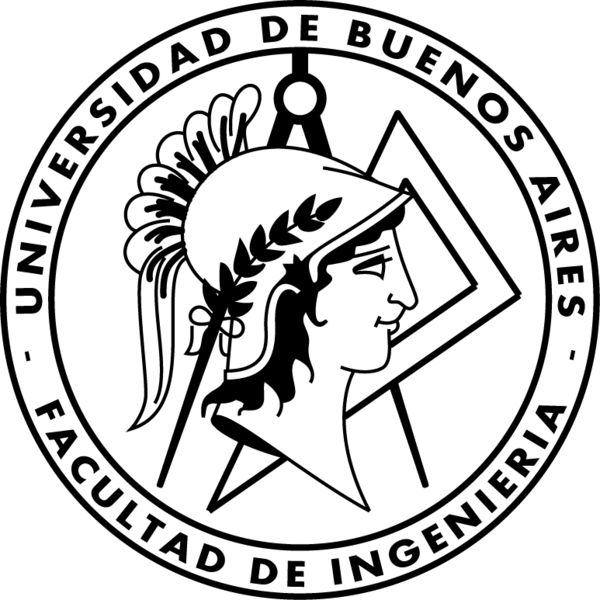
\includegraphics[width=7.5cm, height=7.5cm]{images/logo}
    \end{center}

    \materia{Organización de Datos}
    \submateria{Segundo Cuatrimestre 2017}
    \titulo{Trabajo Práctico 1}

    \integrante{Rodrigo De Rosa}{97799}{rodrigoderosa@outlook.com}
    \integrante{Marcos Schapira}{97934}{schapiramarcos@gmail.com}
    \integrante{Facundo Guerrero}{97981}{facundoiguerrero@gmail.com}
    \maketitle
    %Fin caratula
    %Table of contents
    \newpage
    \pagenumbering{roman}
    \tableofcontents
    %Fin table of contents
    %Informe
    \newpage
	\pagenumbering{arabic}
	\part{Análisis de la variación de precio en el périodo 2013-2017}

		\section{Análisis Global}

      \subsection{Objetivo}

        \tab Esta sección tiene el objetivo de analizar como fueron variando los precios de las distintas propiedades en los últimos 4 años. Con fin introductorio, se quiere brindar una mirada global acerca de la fluctuación de los precios de todas las propiedades a lo largo de los últimos 4 años.

      \subsection{Preparación y procesamiento de los datos}

        \tab Para poder obtener una mejor visualización global de los datos, se tuvieron en cuenta algunas características sobresalientes para filtrar los datos. Como primera aproximación, se recortaron todos los features que no fueran
        de \textit{CABA+GBA}. Por otro lado, se filtraron los features a los cuales no fue posible obtener el precio. Sumado a esto, también fueron filtrados los features a los cuales no se pudo obtener la ubicación geográfica.
        Por otra parte, cabe destacar que el análisis de la variación global que esta próximo a presentarse, fue realizado sobre el precio aproximado de cada propiedad en $usd$. Por último, al tratarse de una primera visión global, esta sección no presenta filtrado por ninguna característica adicional del set de datos.
        \\
        \tab Para procesamiento de los datos, primero se separaron y agruparon los features por años. A continuación, para cada dataframe formado, es decir para las propiedades de un determinado año, lo que se hizo fue separarlas por meses. Entonces hasta el momento tenemos las propiedades separadas por años y por meses. Por último para cada año, se agruparon todas las propiedades de un mismo mes dejando como valor el precio en dolares promedio de las mismas.

      \subsection{Presentación de los gráficos de promedios}

        \tab Aquí se muestran los gráficos que representan los promedios anteriormente mencionados para cada año.
        Vale aclarar que en los siguientes 5 gráficos el eje x representa los meses de cada año, y el eje y representa el precio de las propiedades en usd. Dicho precio varia entre 0$-$450000 $usd$, para obtener una mirada objetiva de los gráficos que serán presentados acontinuación.

				\begin{center}
       				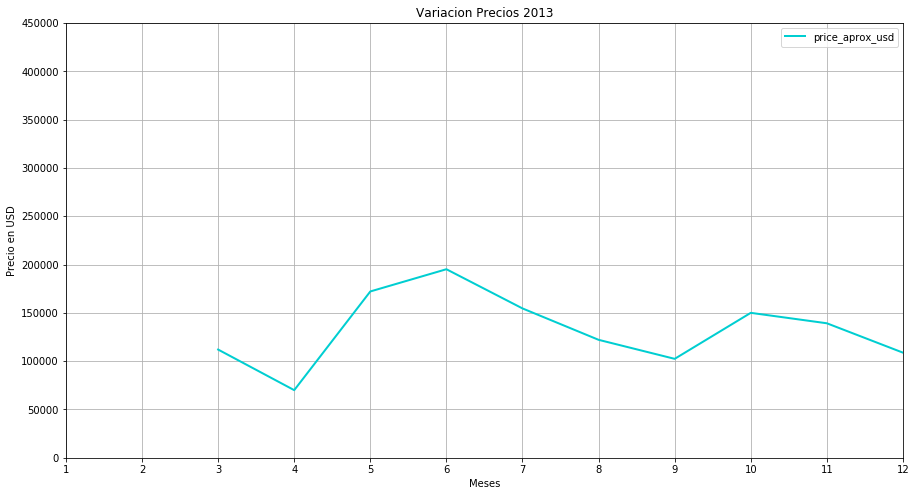
\includegraphics[width=6in, height=4.2in]{images/variacion2013}
		   	\end{center}
        \begin{center}
       				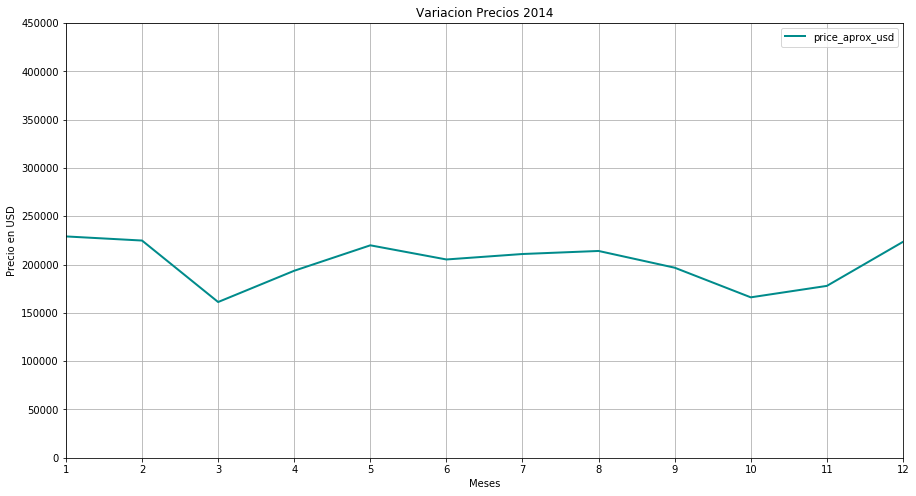
\includegraphics[width=6in, height=4.2in]{images/variacion2014}
		   	\end{center}
        \begin{center}
       				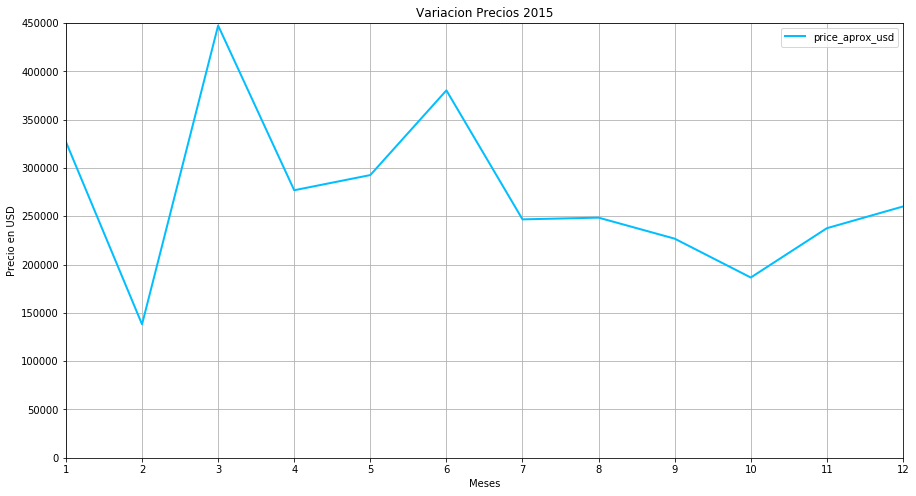
\includegraphics[width=6in, height=4.2in]{images/variacion2015}
		   	\end{center}
        \begin{center}
       				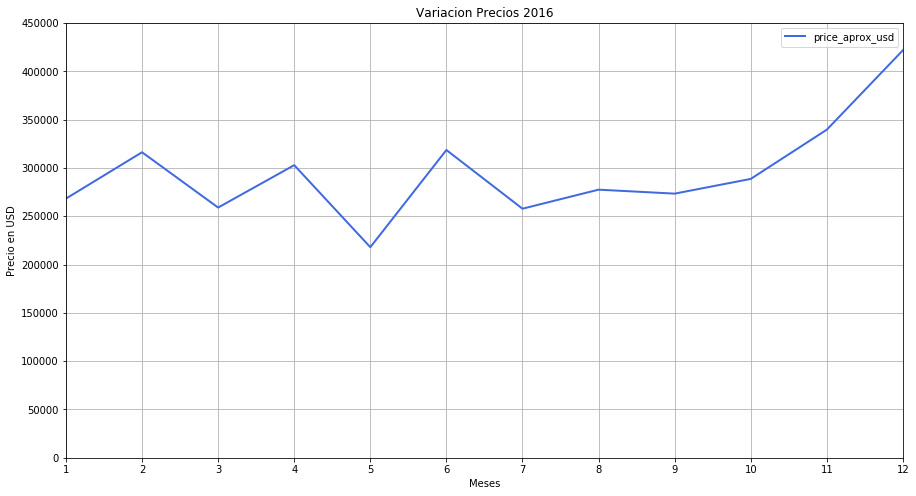
\includegraphics[width=6in, height=4.2in]{images/variacion2016}
		   	\end{center}
        \begin{center}
       				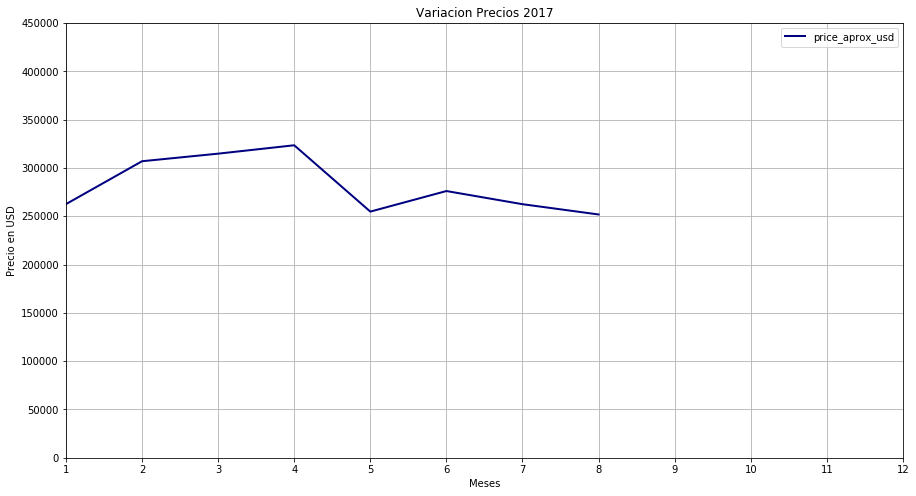
\includegraphics[width=6in, height=4.2in]{images/variacion2017}
		   	\end{center}

      \subsection{Ubicación de las propiedades con mayor precio}

        \tab Luego de presentados los gráficos que representan la fluctuación del precio a través de los años, se procede a presentar una serie de gráficos con el objetivo de analizar la ubicación de las propiedades con mayor precio.
        Para esto, se representa en distintos \code{Heats Map} la ubicación de las propiedades con mayor precio en cada año, es decir que se filtro el mes que poseía un máximo en cada gráfico anterior y se representaron todas las propiedades que estaban en dicho mes.

        \begin{center}
              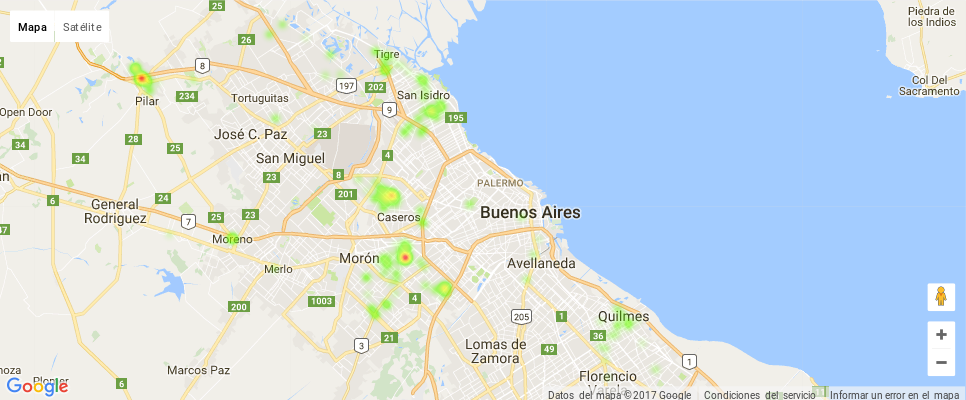
\includegraphics[width=7in, height=4in]{images/ubicP2013}
              \textbf{Gráfico de las propiedades con mayor precio en el 2013.}
        \end{center}
        \begin{center}
              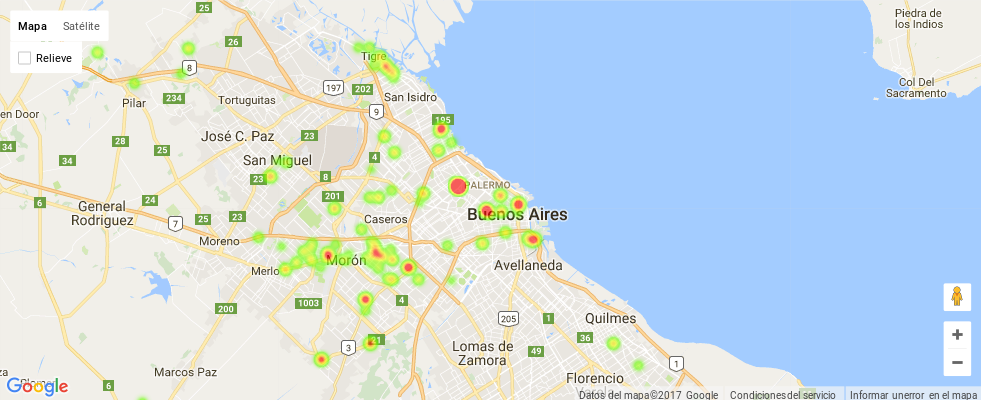
\includegraphics[width=7in, height=4in]{images/ubicP2014}
              \textbf{Gráfico de las propiedades con mayor precio en el 2014.}
        \end{center}
        \begin{center}
              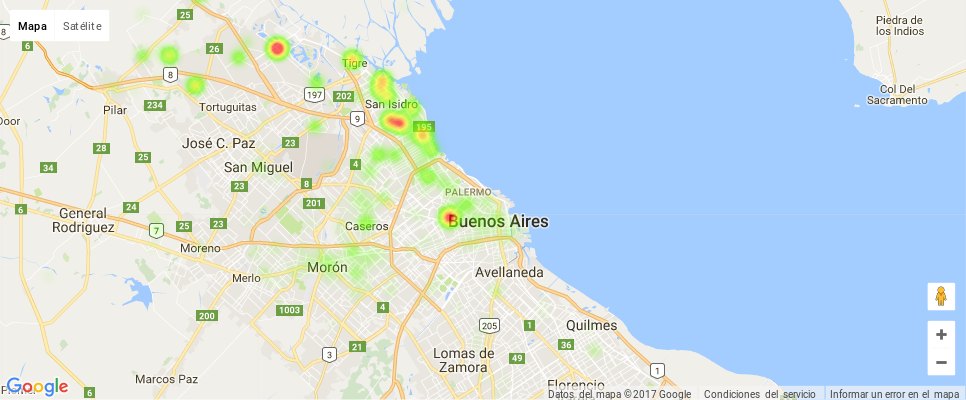
\includegraphics[width=7in, height=4in]{images/ubicP2015}
              \textbf{Gráfico de las propiedades con mayor precio en el 2015.}
        \end{center}
        \begin{center}
              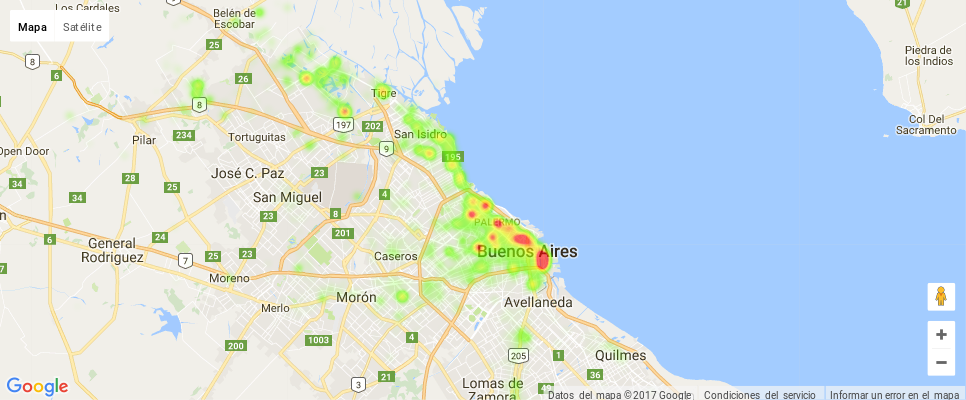
\includegraphics[width=7in, height=4in]{images/ubicP2016}
              \textbf{Gráfico de las propiedades con mayor precio en el 2016.}
        \end{center}
        \begin{center}
              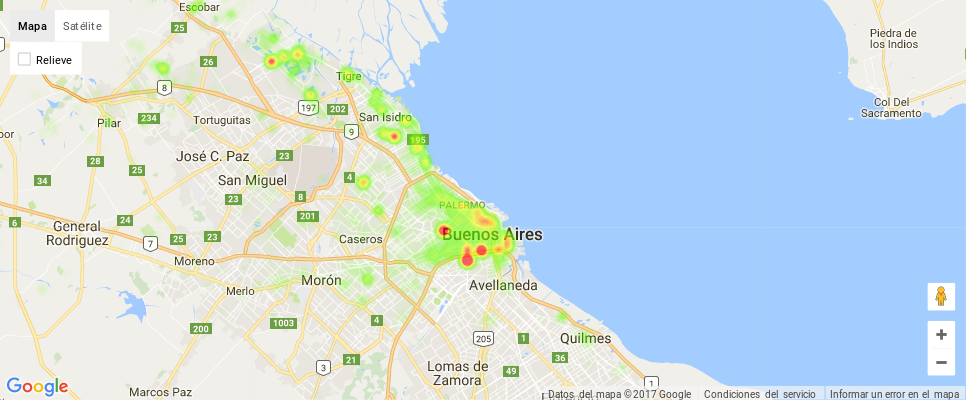
\includegraphics[width=7in, height=4in]{images/ubicP2017}
              \textbf{Gráfico de las propiedades con mayor precio en el 2017.}
        \end{center}


      \subsection{Conclusiones}

        \tab De los gráficos de promedios presentados anteriormente, se pueden visualizar rápidamente  los meses con mayor y menor precio de propiedades en cada año. Se presenta una tabla con dichos datos:

        \begin{center}
          \begin{tabular}{ |c|c|c| }
            \hline
            \multicolumn{3}{|c|}{Limites de precios por años.}\\
            \hline
            \hline
            Año & Mes con Mayor Precio & Mes con menor Precio \\
            \hline
            2013 & Junio & Abril \\
            2014 & Enero & Marzo \\
            2015 & Marzo & Febrero \\
            2016 & Diciembre & Mayo \\
            2017 & Abril & Agosto \\
            \hline
          \end{tabular}
        \end{center}

        \tab Cabe mencionar que estos son los datos que fueron filtrados para poder realizar los \code{Heats Map}.
        Por otra parte, se puede ver en la tabla presentada anteriormente que no se puede sugerir una tendencia de meses con mayores-menores precios, ya que los resultados fueron muy variables.
        Con el objetivo de brindar otra mirada de la diferencia general entre los precios de distintos años, se construyo otro gráfico que representa los mismo promedios anteriormente mencionados, pero organizados de distinta manera para poder que puedan ser comparados entre distintos años. A continuación presentamos el gráfico:

        \begin{center}
              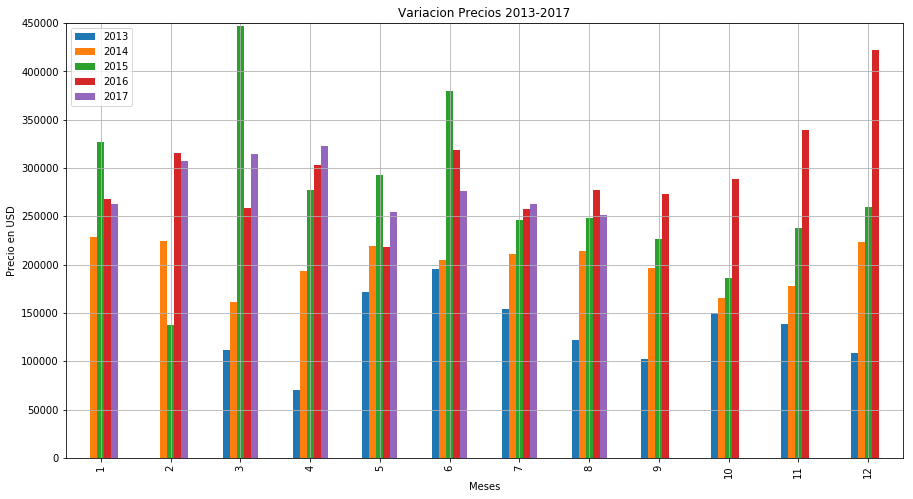
\includegraphics[width=6in, height=4.2in]{images/comparacionAnual}
        \end{center}

        \tab Como se menciono anteriormente, este gráfico tiene la finalidad de poder brindar una mirada global de los precios a lo largo de los años. Como se puede ver, tenemos en el eje x los meses y para cada mes representamos los 5 años a analizar. Observando detenidamente, se pueden extraer muchas conclusiones.
        Lo primero y mas sencillo de ver son los meses con mayor y menor precio de los 5 años. Se puede observar que el mes de Marzo del 2015 fue el que tuvo precios mas elevados de ventas, y por el contrario, el mes de Abril del 2013 fue el que tuvo los precios mas bajos en las mismas. Ademas se puede ver que 2013 tuvo menor precio que el resto de los años en todos los meses. Siguiendo la misma linea, es fácil observar que 2014 es el segundo año con menores precios, salvo en febrero que supero a 2015. Por otro lado se puede visualizar que los primeros meses de 2015 fueron muy variantes, teniendo su mínimo en febrero y máximo en marzo, pero a partir de Junio-Julio se establece una media que supera a los 2 años anteriormente mencionados. Por último se puede ver que el año 2016 en la primera mitad posee precios que se sitúan entre los mas elevados, y en la segunda mitad establece una tendencia creciente la cual supera al resto de los años.
       \\
       \tab Todo esto de cierta forma permite inferir, que a medida que se avanza en los años las propiedades que fueron vendidas poseían precios mayores a la de años anteriores.
       \\
       \tab Por otra parte, siguiendo el análisis recientemente hecho, se puede observar una cierta tendencia en los \code{Heats Maps} presentados anteriormente. En dichos gráficos se puede notar que en los primeros años hay un predominio de propiedades en \textit{Zona Norte} y \textit{Zona Oeste} del \textit{Gran Buenos Aires}, pero a medida que avanzan los años podemos notar un corrimiento hacia \textit{CABA}, para que finalmente en los últimos 2 años pase a tener un dominio sobre las propiedades con mayor precio. Ademas, a esto le podemos sumar el análisis realizado en la sección( \textbf{PONER SECCION DEL ANALISIS} ), sobre los barrios con mayor \code{Precio por m$^2$}. En ese análisis se obtuvo que los barrios con mayor valor de metro cuadrado, están ubicados en \textit{CABA}, y mas precisamente, están ubicados en la zona que los últimos 2 \code{Heats Maps} nos indican mayor precio en las propiedades.
       \\
       \tab Entonces se infiere que una de las causas del aumento de precios analizado anteriormente, podría ser el corrimiento de las propiedades vendidas hacia \textit{CABA}, dado que allí se encuentran las propiedades con mayor precio de metro cuadrado, y con mayor precio total.

  \section{Análisis dependiendo del tipo de propiedad}

    \subsection{Objetivo}
      \tab Esta sección basa el análisis de la variación de los precios de los distintos tipos de propiedades, siendo estos: \code{$Casas$}, \code{$Departamentos$} y \code{$PH$}.

    \subsection{Preparación y procesamiento de los datos}
      \tab La preparación de los datos para esta sección, es la misma que la de la sección anterior con el agregado de que inicialmente se filtra por 1 de los 3 tipos de propiedades mencionados anteriormente. Entonces, para cada sección de las que se presentaran a continuación se tendrá un dataframe solamente con el tipo de vivienda que se este analizando.

    \subsection{Análisis de la variación de precios de las casas}

      \tab Esta sección basa su análisis sobre la variación del precio de las \code{casas}. Lo que se hizo, fue filtrar el dataframe para todas las propiedades que sean de tipo casa.

      \subsubsection{Presentación de los gráficos promedios}

        \tab Al igual que en el análisis global de las propiedades, se presentaran gráficos que representan los promedios mensuales de las propiedades de tipo \code{casa} para cada año. En los siguientes gráficos, al igual que en el análisis global, el eje x representa los meses de cada año, y el eje y representa el precio de las propiedades en usd. Dicho precio varia entre 0$-$600000 $usd$.

        \begin{center}
              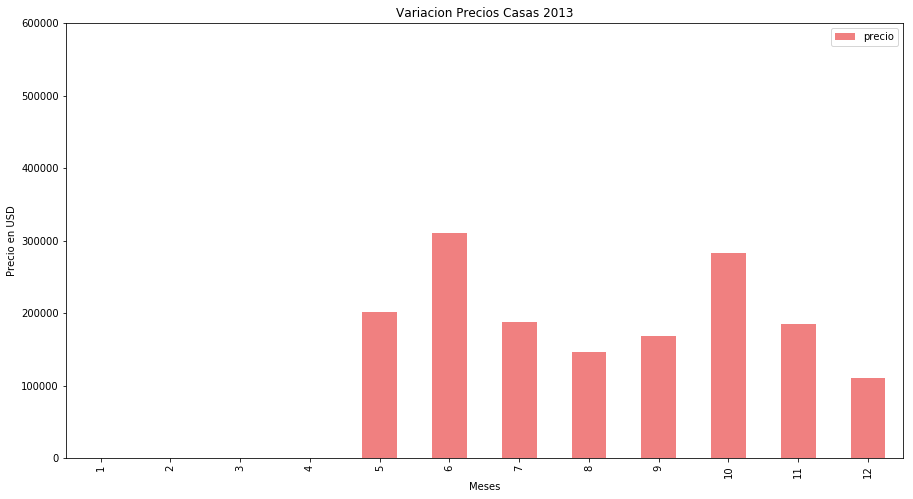
\includegraphics[width=6in, height=4.2in]{images/vCasas2013}
        \end{center}
        \begin{center}
              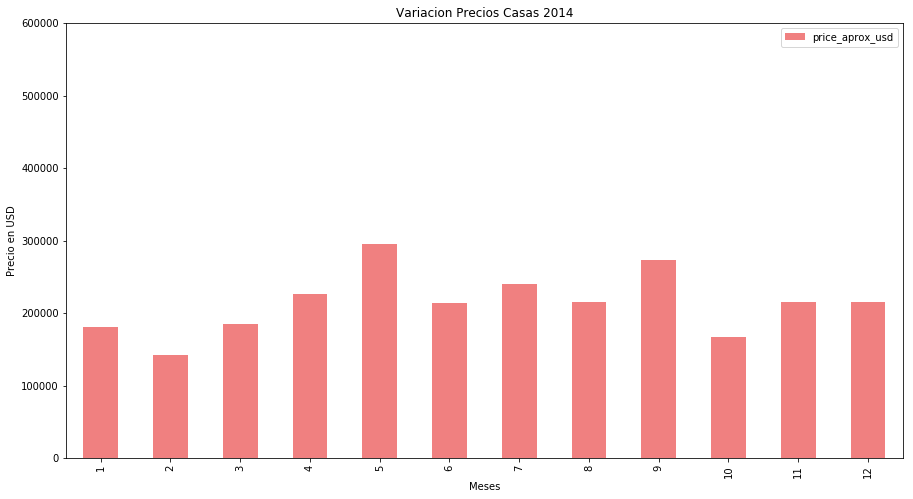
\includegraphics[width=6in, height=4.2in]{images/vCasas2014}
        \end{center}
        \begin{center}
              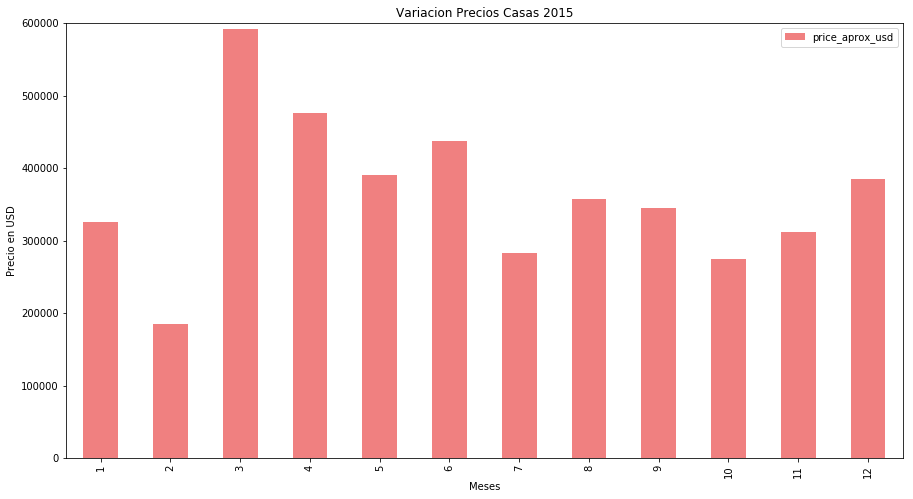
\includegraphics[width=6in, height=4.2in]{images/vCasas2015}
        \end{center}
        \begin{center}
              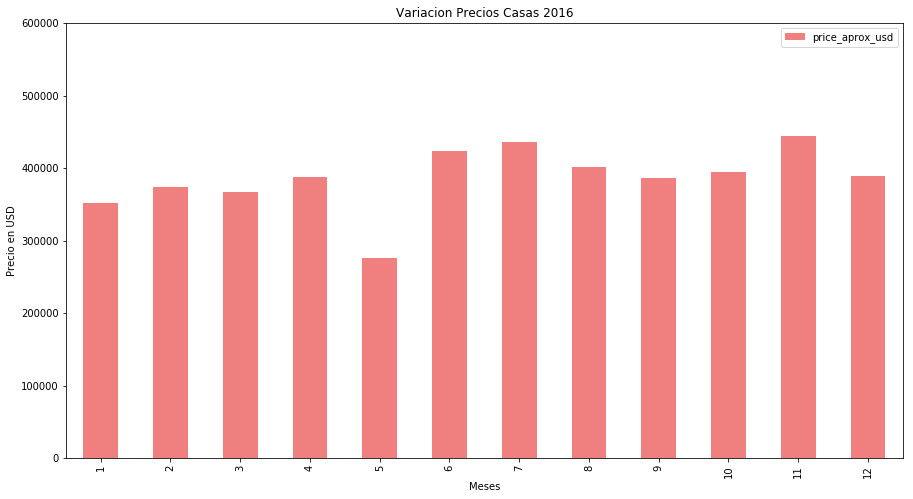
\includegraphics[width=6in, height=4.2in]{images/vCasas2016}
        \end{center}
        \begin{center}
              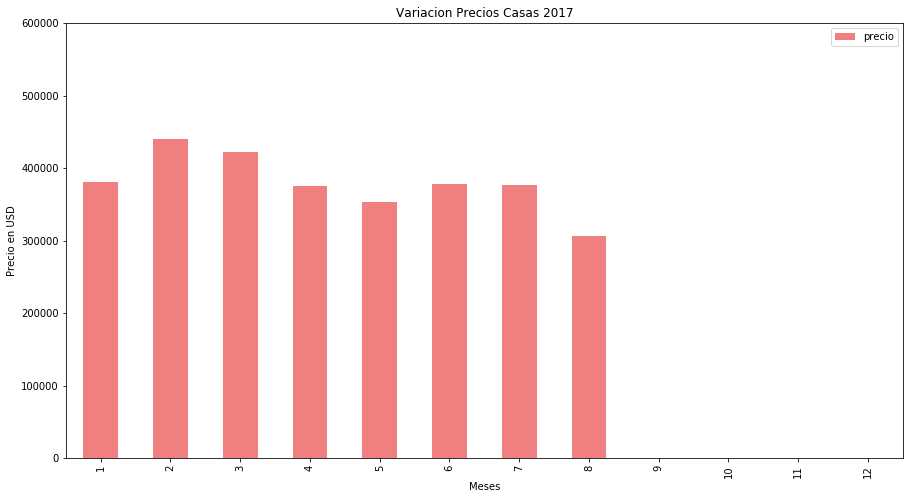
\includegraphics[width=6in, height=4.2in]{images/vCasas2017}
        \end{center}

      \subsubsection{Ubicaciones de las Casas}

        \tab Ahora se presentara un \code{Heat Map} que pretende mostrar la localización de las casas para todos los años.

        \begin{center}
              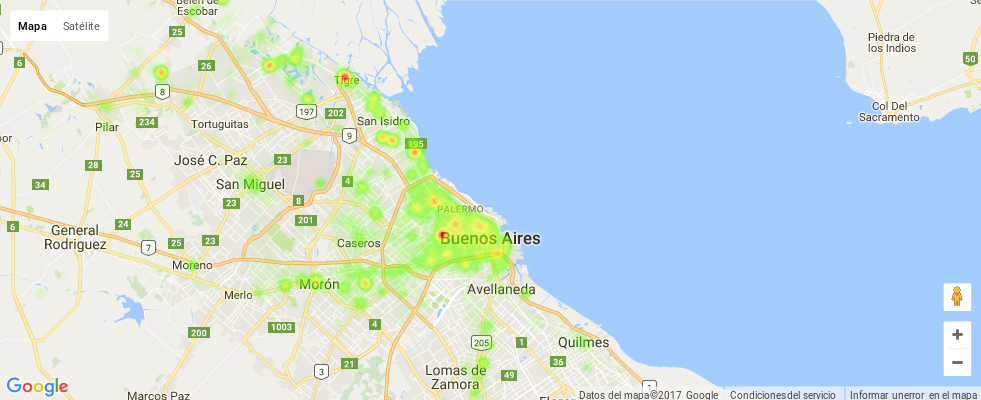
\includegraphics[width=7in, height=4in]{images/ubicCasas}
              \textbf{Gráfico de la ubicación de las casas entre 2013-2017.}
        \end{center}

      \subsubsection{Conclusiones de la variación de precios de las casas}

        \tab Como se puede observar, los gráficos promedios de la variación de precio de las casas siguen una tendencia similar a la analizada globalmente. Algo importante a destacar, es el cambio brusco de los precios entre los meses Febrero-Marzo del año 2015. Al igual que en el análisis global, estos son los meses con menores y mayores precios de casas vendidas del año 2015 respectivamente. Sumando a esto, tambien es importante destacar que en el caso particular de las casas, no se puede apreciar la tendencia creciente que se observa en la segunda mitad del año 2016.
        \\
        \tab Por otro lado se puede ver en el \code{Heat Map} presentado anteriormente que hay una dominio de \textit{CABA} en la ubicación de las casas, pero tambien es para destacar que \textit{Zona Norte} posee una gran proporción de casas.

    \subsection{Análisis de la variación de precios de los Departamentos}

      \tab Esta sección basa su análisis sobre la variación del precio de los \code{departamentos}. Lo que se hizo, fue filtrar el dataframe para todas las propiedades que sean de tipo departamento.

      \subsubsection{Presentación de los gráficos promedio}
        \tab Al igual que en la sección anterior, se presentan los gráficos que representan el promedio mensual del valor de los \code{Departamentos} para todos los años. En este caso, la escala tomada para el eje y varia entre 0$-$500000 $usd$.

        \begin{center}
              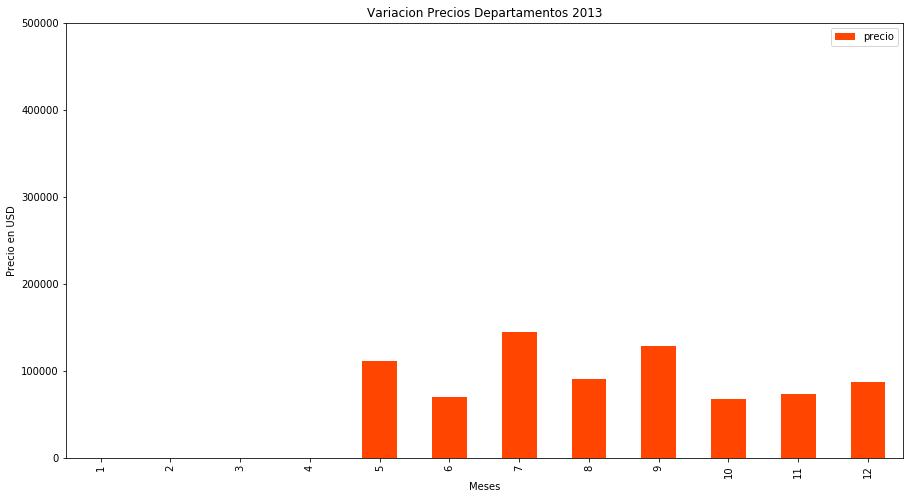
\includegraphics[width=6in, height=4.2in]{images/vDeptos2013}
        \end{center}
        \begin{center}
              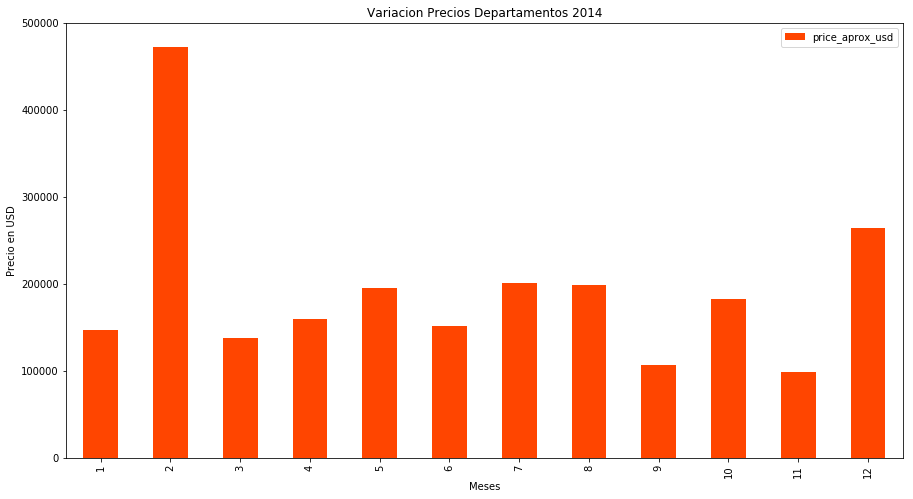
\includegraphics[width=6in, height=4.2in]{images/vDeptos2014}
        \end{center}
        \begin{center}
              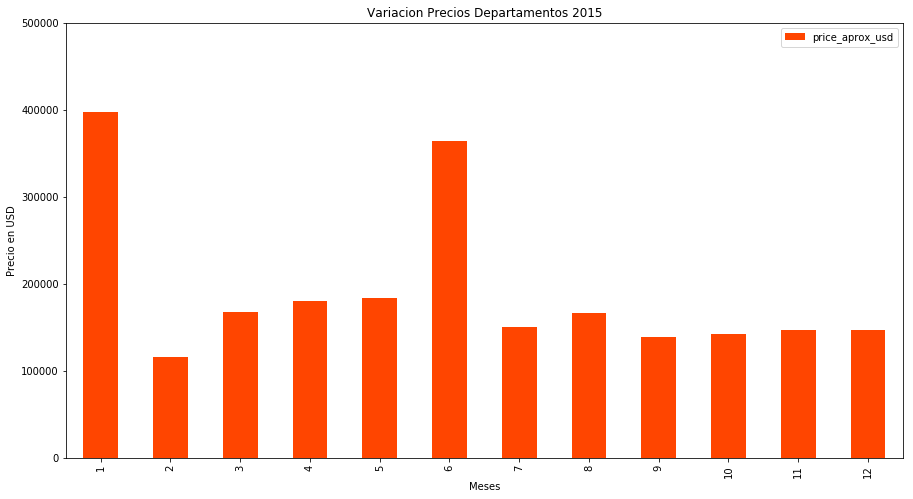
\includegraphics[width=6in, height=4.2in]{images/vDeptos2015}
        \end{center}
        \begin{center}
              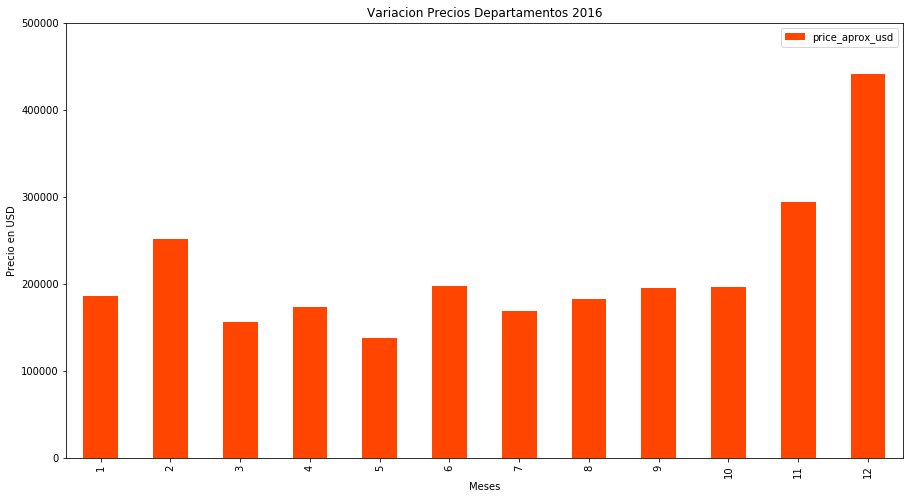
\includegraphics[width=6in, height=4.2in]{images/vDeptos2016}
        \end{center}
        \begin{center}
              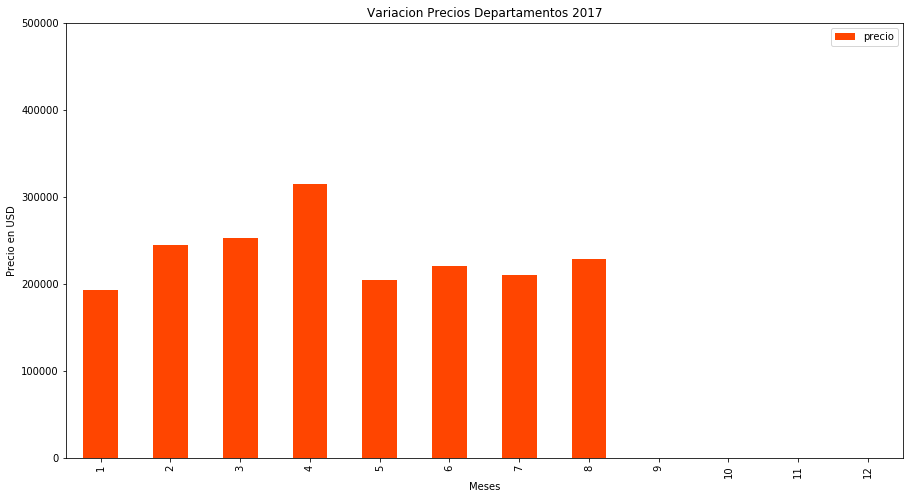
\includegraphics[width=6in, height=4.2in]{images/vDeptos2017}
        \end{center}

      \subsubsection{Ubicaciones de los Departamentos}

        \tab Aquí se adjuntara un \code{Heat Map} que mostrara la ubicación de los departamentos para todos los años.

        \begin{center}
              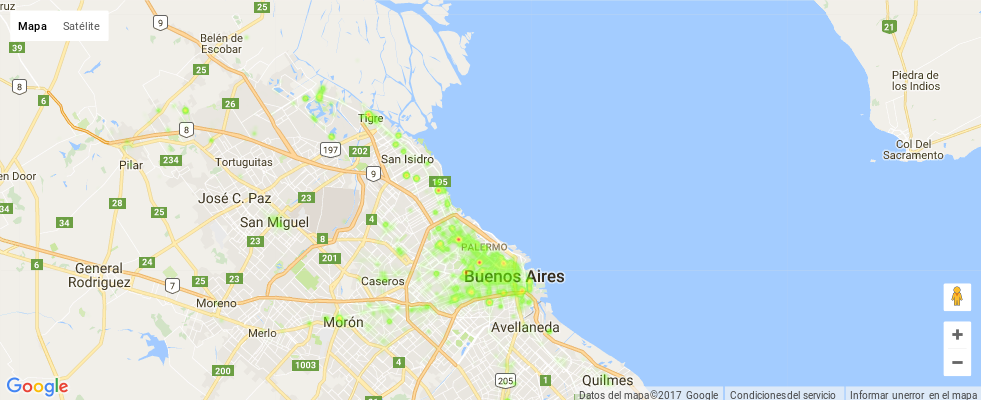
\includegraphics[width=7in, height=4in]{images/ubicDeptos}
              \textbf{Gráfico de la ubicación de los departamentos entre 2013-2017.}
        \end{center}

      \subsubsection{Conclusiones de la variación de precios de los Departamentos}

        \tab Como se puede notar, en los primeros 3 años los gráficos promedios de la variación de precio de los departamentos no siguen la tendencia global analizada anteriormente. Por ejemplo, en Febrero de 2014 se tiene un pico de casi 500 mil $usd$ para los departamentos, mientras que en la tendencia global, el mes de febrero no llega a la mitad de ese valor. También, se puede observar que el brusco cambio de precios de los meses Febrero-Marzo del 2015 visto en el análisis global, no se encuentra presente en los departamentos. De todas formas, en los últimos 2 años se adecua a las tendencias globales establecidas. Algo importante a destacar, es que al igual que en el análisis global, se puede apreciar la tendencia creciente de la segunda mitad del año 2016.
        \\
        \tab Por otro lado se puede observar en el \code{Heat Map} adjuntado anteriormente que hay una total centralización de los departamentos en la zona de \textit{CABA}, lo cual es totalmente razonable debido al nivel de edificación de la zona.


	\subsection{Análisis de la variación de precios de los PH}

  \subsubsection{Presentación de los gráficos promedio}
    \tab Al igual que en las 2 secciónes anteriores, se presentan los gráficos que representan el promedio mensual del valor de los \code{PH} para todos los años:

    \begin{center}
          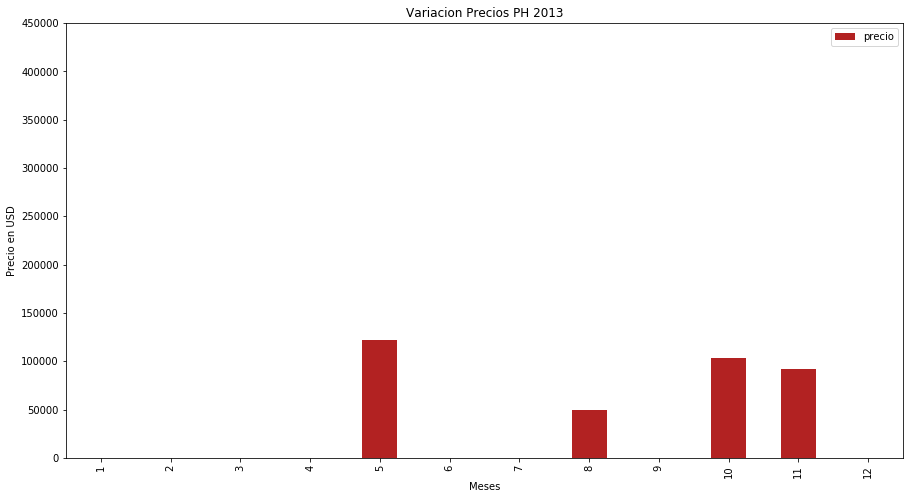
\includegraphics[width=6in, height=4.2in]{images/vPH2013}
    \end{center}
    \begin{center}
          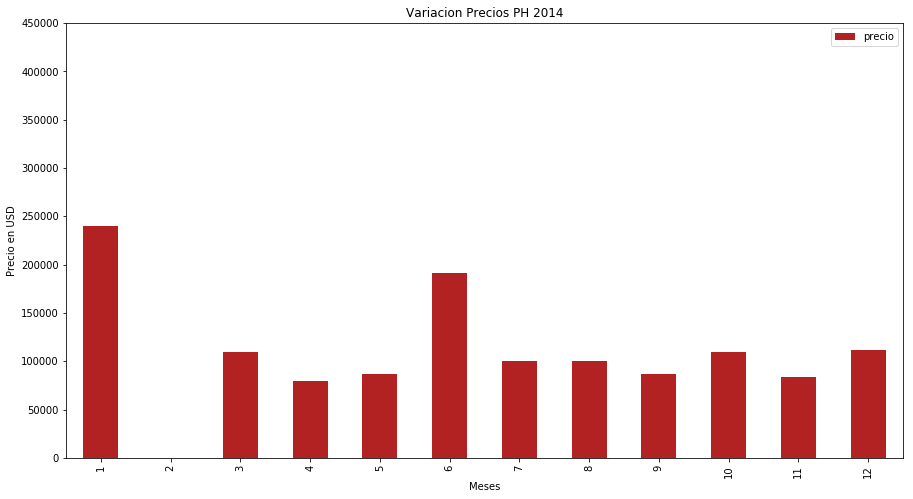
\includegraphics[width=6in, height=4.2in]{images/vPH2014}
    \end{center}
    \begin{center}
          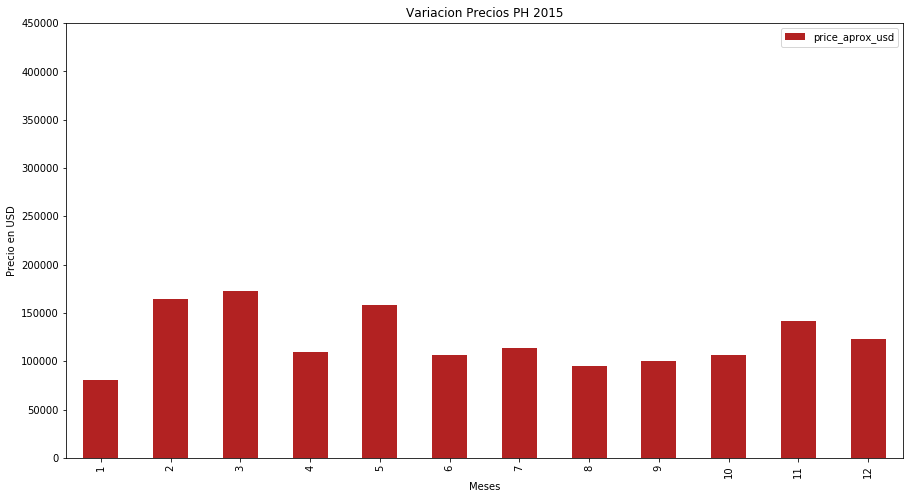
\includegraphics[width=6in, height=4.2in]{images/vPH2015}
    \end{center}
    \begin{center}
          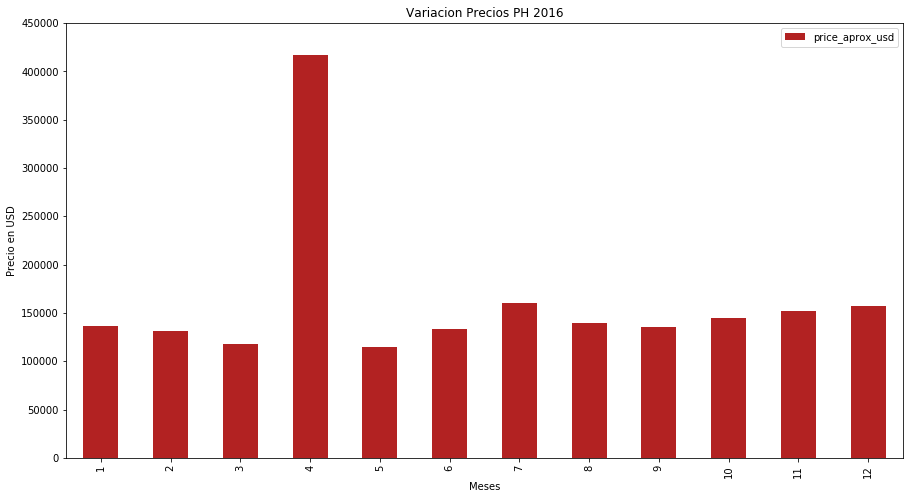
\includegraphics[width=6in, height=4.2in]{images/vPH2016}
    \end{center}
    \begin{center}
          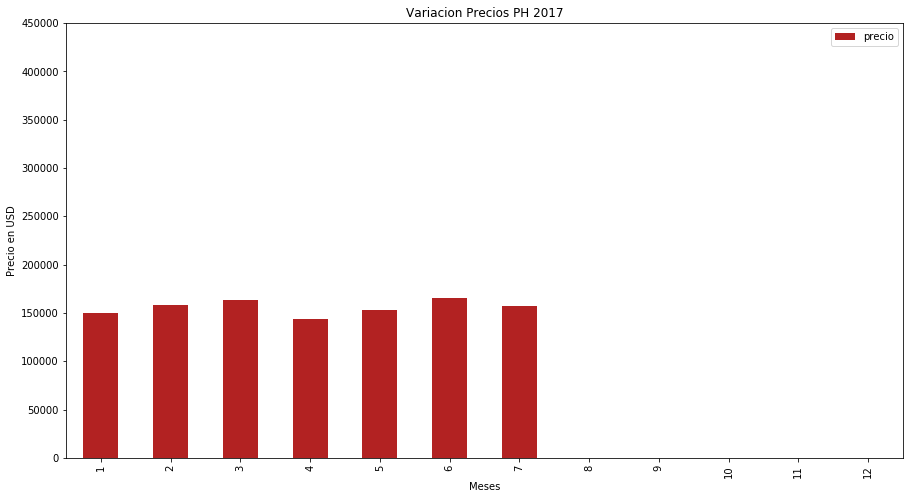
\includegraphics[width=6in, height=4.2in]{images/vPH2017}
    \end{center}

  \subsubsection{Ubicaciones de los PH}

    \tab Aquí se adjuntara un \code{Heat Map} que mostrara la ubicación de los departamentos para todos los años.

    \begin{center}
          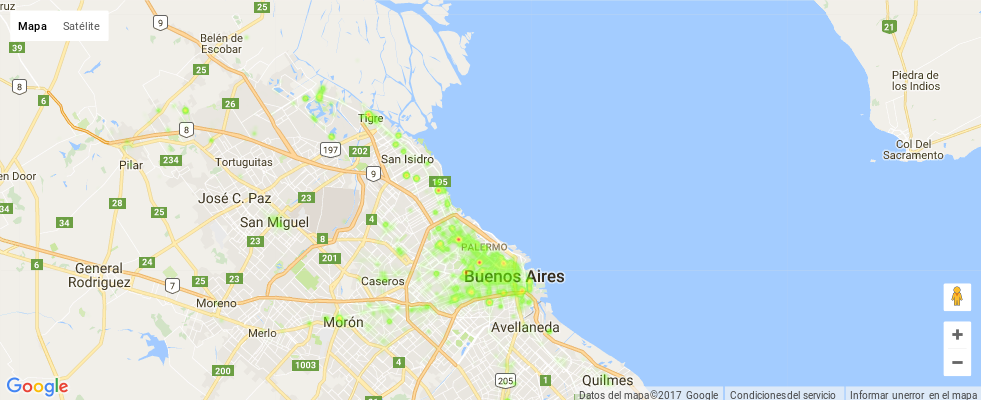
\includegraphics[width=7in, height=4in]{images/ubicDeptos}
          \textbf{Gráfico de la ubicación de los departamentos entre 2013-2017.}
    \end{center}

  \subsubsection{Conclusiones de la variación de precios de los PH}

    \tab Como se puede notar, en los primeros 3 años los gráficos promedios de la variación de precio de los departamentos no siguen la tendencia global analizada anteriormente. Por ejemplo, en Febrero de 2014 se tiene un pico de casi 500 mil $usd$ para los departamentos, mientras que en la tendencia global, el mes de febrero no llega a la mitad de ese valor. También, se puede observar que el brusco cambio de precios de los meses Febrero-Marzo del 2015 visto en el análisis global, no se encuentra presente en los departamentos. De todas formas, en los últimos 2 años se adecua a las tendencias globales establecidas. Algo importante a destacar, es que al igual que en el análisis global, se puede apreciar la tendencia creciente de la segunda mitad del año 2016.
    \\
    \tab Por otro lado se puede observar en el \code{Heat Map} adjuntado anteriormente que hay una total centralización de los


\end{document}
